\begin{center}
	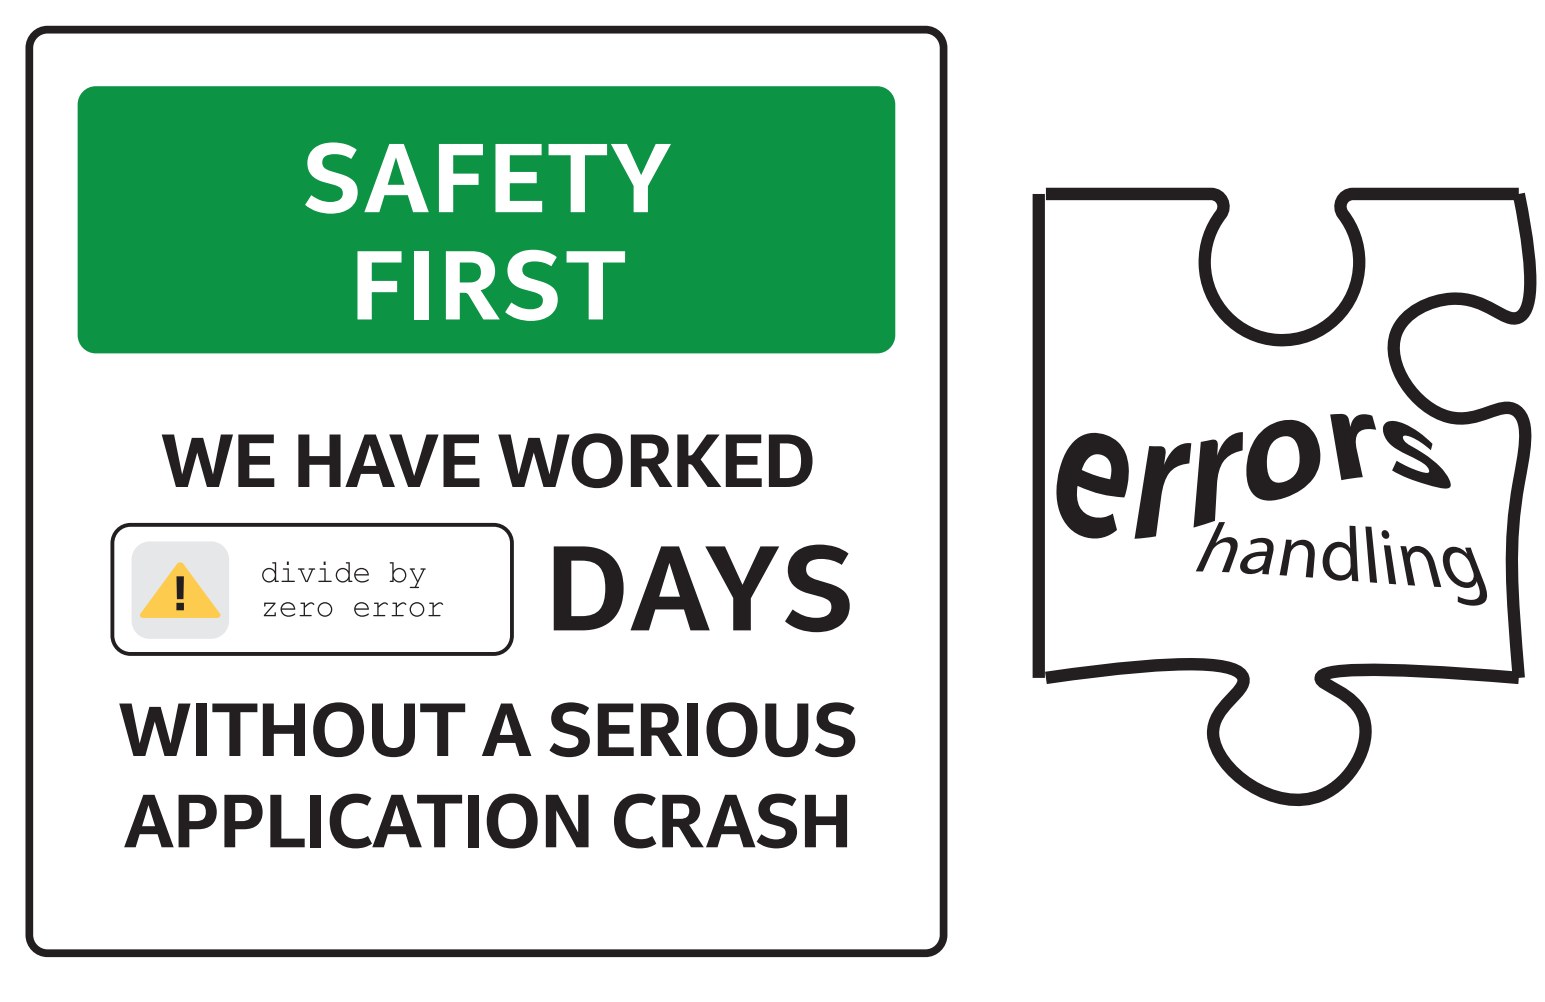
\includegraphics[width=0.5\textwidth]{content/chapter-5/images/1}
\end{center}

Agatha Christie wrote in 1969 that “human error is nothing to what a computer can do if it tries.” It is no mystery that we, as programmers, get to clean up the mess. The mechanisms for error handling could catch programmer errors that others may make. Since we do not plan on making mistakes ourselves, we can focus on using error handling to handle conditions that may occur in the real world from other causes.\par

Detecting and dealing with unexpected conditions and errors can be helpful during application development (think: the other programmer who works on the project who does make mistakes), but more importantly play a critical role in stable and safe production applications and libraries. We devote this chapter to describing the error handling mechanisms available in SYCL so that we can understand what our options are and how to architect applications if we care about detecting and managing errors.\par

This chapter overviews synchronous and asynchronous errors in SYCL, describes the behavior of an application if we do nothing in our code to handle errors, and dives into the SYCL-specific mechanism that allows us to handle asynchronous errors.\par